\chapter{Modelo Estrutural Causal (SCM)}
\label{cap:dag}

No \cref{cap:intro} vimos que 
as relações causais entre variáveis são
essenciais para conseguirmos determinar
o efeito que uma variável pode ter em outra.
Contudo, como podemos especificar
relações causais formalmente?

Como resposta a esta pergunta iremos
definir o Modelo Estrutural Causal (SCM),
que permite especificar formalmente relações causais.
Para tal, será necessário primeiro introduzir
modelos probabilísticos em grafos.
Um curso completo sobre estes modelos 
pode ser encontrado, por exemplo,
em \citet{Maua2022}.
A seguir, estudaremos resultados
essenciais destes modelos.

\section{Elementos de Modelos Probabilísticos em Grafos}

\subsection{Grafo Direcionado}

\begin{definition}
 \label{def:grafo}
 Um \textbf{grafo direcionado}, 
 $\sG = (\sV, \sE)$,
 é composto por um conjunto de vértices,
 $\sV = \{V_1, \ldots, V_n\}$, e
 e um conjunto de arestas,
 $\sE = \{E_1, \ldots, E_m\}$, onde
 cada aresta é um par ordenado de vértices, isto é,
 $E_i \in \sV^2$.
\end{definition}

Para auxiliar nossa intuição sobre a
\cref{def:grafo}, é comum representarmos
o grafo por meio de uma figura.
Nesta, representamos cada vértice por meio de um ponto.
Além disso, para cada aresta, $(V_i, V_j)$,
traçamos uma seta que aponta de $V_i$ para $V_j$.

Por exemplo, considere que os vértices são
$\sV = \{V_1, V_2, V_3\}$ e as arestas são
$\sE = \{(V_1, V_2), (V_1, V_3), (V_2, V_3)\}$.
Neste caso, teremos os $3$ pontos como vértices e,
além disso, traçaremos setas de $V_1$ para $V_2$ e para $V_3$ e,
também, de $V_2$ para $V_3$.
Podemos desenhar este grafo utilizando os
pacotes \textit{dagitty} e \textit{ggdag}
\citep{Barrett2022,Textor2016}:

\begin{knitrout}
\definecolor{shadecolor}{rgb}{0.969, 0.969, 0.969}\color{fgcolor}\begin{kframe}
\begin{alltt}
\hlkwd{library}\hlstd{(dagitty)}
\hlkwd{library}\hlstd{(ggdag)}
\hlkwd{library}\hlstd{(ggplot2)}

\hlcom{# Especificar o grafo}
\hlstd{grafo} \hlkwb{<-} \hlkwd{dagitty}\hlstd{(}\hlstr{"dag \{
    V1 -> \{ V2 V3 \}
    V2 -> V3
\}"}\hlstd{)}

\hlcom{# Exibir a figura do grafo}
\hlkwd{ggdag}\hlstd{(grafo,} \hlkwc{layout} \hlstd{=} \hlstr{"circle"}\hlstd{)} \hlopt{+}
  \hlkwd{theme}\hlstd{(}\hlkwc{axis.text.x}\hlstd{=}\hlkwd{element_blank}\hlstd{(),}
      \hlkwc{axis.ticks.x}\hlstd{=}\hlkwd{element_blank}\hlstd{(),}
      \hlkwc{axis.text.y}\hlstd{=}\hlkwd{element_blank}\hlstd{(),}
      \hlkwc{axis.ticks.y}\hlstd{=}\hlkwd{element_blank}\hlstd{())} \hlopt{+}
  \hlkwd{xlab}\hlstd{(}\hlstr{""}\hlstd{)} \hlopt{+} \hlkwd{ylab}\hlstd{(}\hlstr{""}\hlstd{)}
\end{alltt}
\end{kframe}\begin{figure}[t]

{\centering 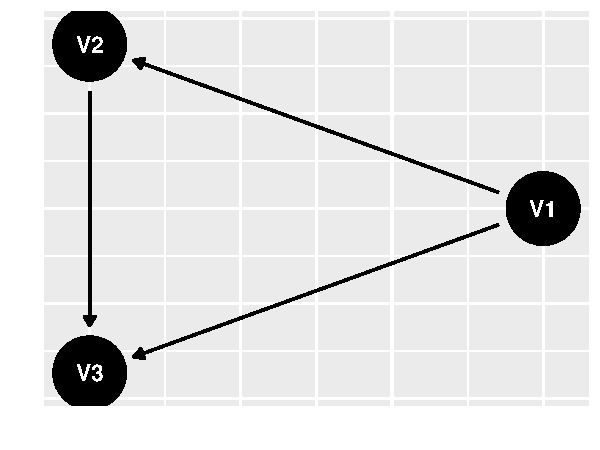
\includegraphics[width=\maxwidth]{figure/grafo1-1} 

}

\caption[Exemplo de grafo]{Exemplo de grafo.}\label{fig:grafo1}
\end{figure}

\end{knitrout}

Grafos direcionados serão úteis para 
representar causalidade pois 
usaremos vértices para representar variáveis e
arestas para apontar de 
cada causa imediata para seu efeito.
Por exemplo, no \Cref{cap:intro}
consideramos um caso em que Sexo e Tratamento são
causas imediatas de recuperação e, além disso,
Sexo é causa imediata de Tratamento.
O grafo na \cref{fig:grafo1} poderia
representar estas relações se definirmos que
$V_1$ é Sexo, $V_2$ é Tratamento e 
$V_3$ é Recuperação.

Usando a representação de um grafo,
podemos imaginar caminhos sobre ele.
Um \textbf{caminho direcionado} inicia-se 
em um determinado vértice e, 
seguindo a direção das setas, 
vai de um vértice para outro.
Por exemplo, $(V_1, V_2, V_3)$ é
um caminho direcionado na 
\cref{fig:grafo1}, pois existe
uma seta de $V_1$ para $V_2$ e
de $V_2$ para $V_3$.
É comum denotarmos este caminho direcionado por
$V_1 \rightarrow V_2 \rightarrow V_3$.
Similarmente, $(V_1, V_3, V_2)$ não é
um caminho direcionado, pois
não existe seta de $V_3$ para $V_2$.
A definição de caminho direcionado é
formalizada a seguir:

\begin{definition}
 \label{lem:caminhodir}
 Um \textbf{caminho direcionado} é 
 uma sequência de vértices em
 um grafo direcionado,
 $C = \{V_1, \ldots, V_n\}$ tal que, 
 para cada $1 \leq i < n$,
 $(V_i, V_{i+1}) \in \sE$.
\end{definition}

\begin{definition}
 \label{def:descendente}
 Dizemos que $V_2$ é descendente de $V_1$ se
 existe um caminho direcionado de $V_1$ em $V_2$.
\end{definition}

Um \textit{caminho} é uma generalização 
de caminho direcionado.
Em um caminho, começamos em um vértice e,
seguindo por setas, mas 
não necessariamente na direção 
em que elas apontam, vamos
de um vértice para outro.
Por exemplo, na \cref{fig:grafo1}
vimos que $(V_1, V_3, V_2)$ não é um 
caminho direcionado pois não existe seta de $V_3$ para $V_2$.
Contudo, $(V_1, V_3, V_2)$ é um caminho pois
existe uma seta ligando $V_3$ e $V_2$,
a seta que aponta de $V_2$ para $V_3$.
É comum representarmos este caminho por
$V_1 \rightarrow V_3 \leftarrow V_2$.
Caminho é formalizado a seguir:

\begin{definition}
 \label{def:caminho}
 Um \textbf{caminho} é uma sequência de vértices,
 $C = \{V_1, \ldots, V_n\}$ tal que, 
 para cada $1 \leq i < n$,
 $(V_i, V_{i+1}) \in \sE$ ou 
 $(V_{i+1}, V_{i}) \in \sE$. 
\end{definition}

\subsection{Grafo Direcionado Acíclico (DAG)}

Um DAG é um grafo direcionado tal que,
para todo vértice, $V$, não é possível
seguir setas partindo de $V$ e
voltar para $V$. Este conceito é
formalizado a seguir:

\begin{definition}
 \label{def:dag}
 Um \textbf{grafo direcionado acíclico} (DAG) é
 um grafo direcionado, $\sG$,
 tal que, para todo
 vértice, $V \in \sV$, não existe um
 caminho direcionado, $C = \{V_1, \ldots, V_n\}$
 tal que $V_1 = V = V_n$.
\end{definition}

Usualmente representaremos
as relações causais por meio de um DAG.
Especificamente, existirá uma aresta de $V_1$ para $V_2$
para indicar que $V_1$ é causa imediata de $V_2$.
Caso um grafo direcionado não seja um DAG,
então existe um caminho de $V$ em $V$, isto é,
$V$ seria uma causa de si mesma, 
o que desejamos evitar.

Um DAG induz uma \textit{ordem parcial} entre 
os seus vértices. Isto é,
se existe uma aresta de $V_1$ para $V_2$,
então podemos interpretar que
$V_1$ antecede $V_2$ causalmente.
Com base nesta ordem parcial, é
possível construir diversas
definições que nos serão úteis.

Dizemos que $V_1$ é pai de $V_2$ em
um DAG, $\sG$, se
existe uma aresta de $V_1$ a $V_2$,
isto é, $(V_1, V_2) \in \sE$.
Denotamos por $Pa(V)$ o
conjunto de todos os pais de $V$:

\begin{definition}
 \label{def:pais}
 Em um DAG, $\sG$,
 o conjunto de \textbf{pais} de $V \in \sV$, $Pa(V)$, é:
 $$Pa(V) = \{V^* \in \sV: (V^*, V) \in \sE\}.$$
\end{definition}

Similarmente, dizemos que $V_1$ é um ancestral de $V_2$ em
um DAG, se $V_1$ antecede $V_2$ causalmente. Isto é,
se $V_1$ é pai de $V_2$ ou, pai de pai de $V_2$, ou
pai de pai de pai de $V_2$, e assim por diante $\ldots$
Denotamos por $Anc(\V)$ o conjunto de 
todos os ancestrais de elementos de $\V$:

\begin{definition}
 \label{def:ancestrais}
 Em um DAG, $\sG$,
 o conjunto de \textbf{ancestrais} de $\V \subseteq \sV$, 
 $Anc(\V)$, é tal que
 $Anc(\V) \subseteq \sV$ e
 $V^* \in Anc(\V)$ se e somente se existe
 $V \in \V$ e
 um caminho direcionado em $\sG$, C, tal que
 $C_1 = V^*$ e, para algum i, $C_i = V$.
\end{definition}

Note que podemos interpretar $Anc(\V)$ como
o conjunto de todas as causas diretas e indiretas de $\V$.

Finalmente, diremos que um conjunto de vértices,
$\sA \subseteq \sV$ é \textit{ancestral} em um DAG,
se não existe algum vértice fora de $\sA$ que
seja pai de algum vértice em $\sA$.
Segundo nossa interpretação causal,
$\sA$ será ancestral quando 
nenhum vértice fora de $\sA$ 
é causa direta de 
algum vértice em $\sA$:

\begin{definition}
 \label{def:ancestral}
 Em um DAG, $\sG$,
 dizemos que $\sA \subseteq \sV$ é \textbf{ancestral} se,
 para todo $V \in \sA$, temos que
 $Pa(V) \subseteq \sA$.
\end{definition}

\begin{lemma}
 \label{lem:anc}
 Em um DAG, $\sG$,
 para todo $\V \subseteq \sV$, 
 $Anc(\V)$ é ancestral.
\end{lemma}

\subsection{Modelo Probabilístico em um DAG}

Um modelo probabilístico em um DAG é
tal que cada um dos vértices é uma variável aleatória.
O DAG será usada para descrever 
relações de independência condicional existentes entre
estas variáveis.
Mais especificamente, cada vértice será
independente dos demais vértices dados os seus pais.
Uma maneira alternativa de pensar sobre esta afirmação é
imaginar que cada vértice é gerado somente pelos seus pais.
Esta intuição é formalizada em \cref{def:compativel}:

\begin{definition}
 \label{def:compativel}
 Para $\sV$ um conjunto de variáveis aleatórias,
 dizemos que uma função de densidade sobre $\sV$, 
 $f$, é compatível com um DAG, $\sG$, se:
 $$f(v_1,\ldots,v_n) = \prod_{i=1}^n f(v_i|Pa(v_i))$$
\end{definition}

Na prática, pode ser difícil verificar 
se a \cref{def:compativel} está satisfeita 
Para esses casos,
pode ser útil aplicar o 
\cref{lem:compativel-equiv}:

\begin{lemma}
 \label{lem:compativel-equiv}
 Uma função de densidade, $f$, é
 compatível com um DAG, $\sG$,
 se e somente se, existem funções,
 $g_1,\ldots,g_n$ tais que:
 $$f(v_1,\ldots,v_n) = \prod_{i=1}^n g_i(v_i, Pa(v_i))$$
\end{lemma}

O seguinte lema também é útil

\begin{lemma}
 \label{lem:anc_fat}
 Seja $\sG = (\sV, \sE)$ um DAG.
 Se $\sA$ é ancestral e 
 $f$ é compatível com $\sG$, então
 \begin{align*}
  f(\sA) = \prod_{V \in \sA} f(V|Pa(V))
 \end{align*}
\end{lemma}

A seguir, estudaremos três tipos fundamentais
de modelos probabilísticos em DAG's com
$3$ vértices. 
A intuição obtida a partir destes
exemplos continuará valendo quando
estudarmos grafos mais gerais.

\subsection{Exemplos de Modelo Probabilístico em um DAG}
\label{sec:dag-ex}

Nos exemplos a seguir, considere que
$\sV = (V_1, V_2, V_3)$.

\subsubsection{Confundidor (Confounder)}

No modelo de confundidor, 
as únicas duas arestas são 
$(V_2, V_1)$ e $(V_2, V_3)$.
Uma ilustração de um confundidor
pode ser encontrada 
na \cref{fig:confundidor}.
O modelo de confundidor pode ser usado quando
acreditamos que $V_2$ é uma causa comum a
$V_1$ a $V_3$. Além disso,
$V_1$ não é causa imediata de $V_3$ 
nem vice-versa.

\begin{knitrout}
\definecolor{shadecolor}{rgb}{0.969, 0.969, 0.969}\color{fgcolor}\begin{figure}[t]

{\centering 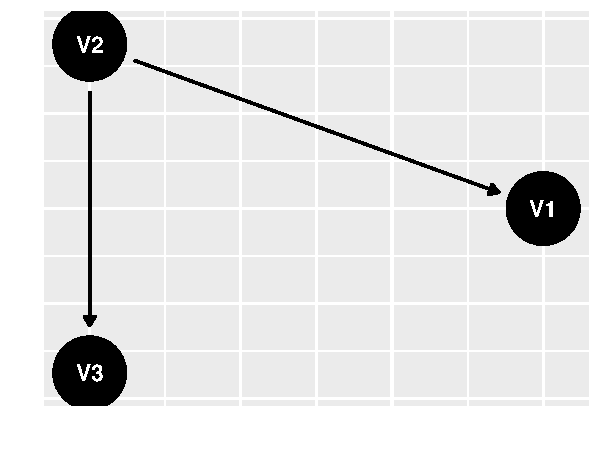
\includegraphics[width=\maxwidth]{figure/confundidor-1} 

}

\caption[Ilustração de confundidor]{Ilustração de confundidor.}\label{fig:confundidor}
\end{figure}

\end{knitrout}

Em um modelo de confundidor 
a relação de dependência entre 
$V_1$ e $V_3$ é explicada pelos
resultados a seguir:

\begin{lemma}
 \label{lem:conf-ind}
 Para qualquer probabilidade compatível com 
 o DAG na \cref{fig:confundidor},
 $V_1 \ind V_3 | V_2$.
\end{lemma}

\begin{proof}
 \begin{align*}
  f(v_1,v_3|v_2) 
  &= \frac{f(v_1,v_2,v_3)}{f(v_2)} \\
  &= \frac{f(v_2)f(v_1|v_2)f(v_3|v_2)}{f(v_2)} 
  & \text{\cref{def:compativel}} \\
  &= f(v_1|v_2)f(v_3|v_2)
 \end{align*}
\end{proof}

\begin{lemma}
 \label{lem:conf-dep}
 Existe ao menos uma probabilidade compatível com
 o DAG na \cref{fig:confundidor} tal que
 $V_1 \not\ind V_3$.
\end{lemma}

\begin{proof}
 Considere que $V_2 \sim \text{Bernoulli}(0.02)$.
 Além disso, $V_1, V_3 \in \{0,1\}$ são independentes dado $V_2$. 
 Também,
 $\P(V_1 = 1|V_2 = 1) = \P(V_3 = 1|V_2 = 1) = 0.9$ e
 $\P(V_1 = 1|V_2 = 0) = \P(V_3 = 1|V_2 = 0) = 0.05$.
 Note que, por construção, $\P$ é 
 compatível com \cref{fig:confundidor}.
 Isto é, $P(v_1,v_2,v_3) = \P(v_2)\P(v_1|v_2)\P(v_3|v_2)$.
 Além disso,
 \begin{align*}
  \P(V_1 = 1) &= \P(V_1 = 1, V_2 = 1) + \P(V_1 = 1, V_2 = 0) \\
              &= \P(V_2=1)\P(V_1=1|V_2=1)
               +\P(V_2=0)\P(V_1=1|V_2=0) \\
              &= 0.02 \cdot 0.9 + 0.98 \cdot 0.05= 0.067
 \end{align*}
 Por simetria, $\P(V_3=1) = 0.067$. Além disso,
 \begin{align*}
  \P(V_1 = 1, V_3 = 1)
  &= \P(V_1 = 1, V_3 = 1, V_2 = 1) 
  +  \P(V_1 = 1, V_3 = 1, V_2 = 0) \\
  &= \P(V_2 = 1)\P(V_1 = 1|V_2 = 1)\P(V_3 = 1|V_2 = 1)
  +  \P(V_2 = 0)\P(V_1 = 1|V_2 = 0)\P(V_3 = 1|V_2 = 0) \\
  &= 0.02 \cdot 0.9 \cdot 0.9 + 0.98 \cdot 0.05 \cdot 0.05 = 0.01865
 \end{align*}
 Como $\P(V_1=1)\P(V_3=1) = 0.067 \cdot 0.067 \approx 0.0045 \neq 0.01865 = \P(V_1=1,V_3=1)$,
 temos que $V_1$ e $V_3$ não são independentes.
\end{proof}

Combinando os \cref{lem:conf-ind,lem:conf-dep} é 
possível compreender melhor como 
usaremos confundidores num contexto causal.
Nestes casos, $V_2$ será uma causa comum a $V_1$ e a $V_3$.
Esta causa comum torna $V_1$ e $V_3$ associados,
ainda que nenhum seja causa direta ou indireta do outro.

Podemos contextualizar estas ideias
em um caso de diagnóstico de dengue.
Considere que 
$V_2$ é a indicadora de que um indivíduo tem dengue, e
$V_1$ e $V_3$ são indicadoras de sintomas típicos de dengue, como
dor atrás dos olhos e febre.
Neste caso, $V_1$ e $V_3$ tipicamente são associados:
caso um paciente tenha febre,
aumenta a probabilidade de que tenha dengue e, portanto,
aumenta a probabilidade de que tenha dor atrás dos olhos.
Contudo, apesar dessa associação 
$V_3$ não tem influência causal sobre $V_1$.
Se aumentarmos a temperatura corporal do indivíduo,
não aumentará a probabilidade de que ele tenha dor atrás dos olhos.
A dengue que causa febre, não o contrário.

\subsubsection{Cadeia (Chain)}

No modelo de cadeia, 
as únicas duas arestas são 
$(V_1, V_2)$ e $(V_2, V_3)$.
Uma ilustração de uma cadeia
pode ser encontrada 
na \cref{fig:cadeia}.
Neste modelo, acreditamos que 
$V_1$ é causa de $V_2$ que,
por sua vez, é causa de $V_3$.
Assim, $V_1$ é ancestral de $V_3$,
isto é, o primeiro é 
causa indireta do segundo.


\begin{knitrout}
\definecolor{shadecolor}{rgb}{0.969, 0.969, 0.969}\color{fgcolor}\begin{figure}[t]

{\centering 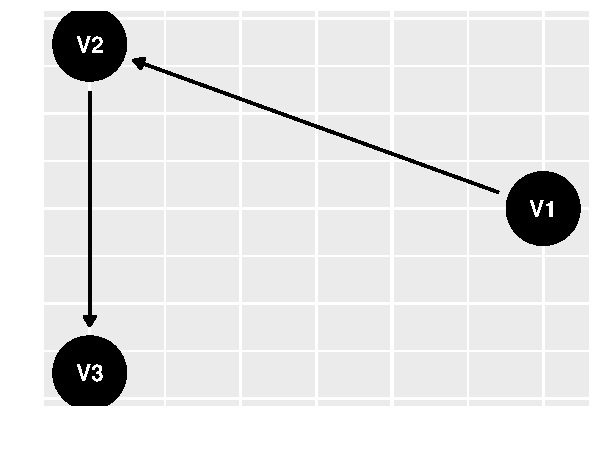
\includegraphics[width=\maxwidth]{figure/cadeia-1} 

}

\caption[Ilustração de cadeia]{Ilustração de cadeia.}\label{fig:cadeia}
\end{figure}

\end{knitrout}

Em um modelo de cadeia 
a relação de dependência entre 
$V_1$ e $V_3$ é explicada pelos
resultados a seguir:

\begin{lemma}
 \label{lem:med-ind}
 Para qualquer probabilidade compatível com 
 o DAG na \cref{fig:cadeia},
 $V_1 \ind V_3 | V_2$.
\end{lemma}

\begin{proof}
 \begin{align*}
  f(v_3|v_1,v_2) 
  &= \frac{f(v_1,v_2,v_3)}{f(v_1,v_2)} \\
  &= \frac{f(v_1)f(v_2|v_1)f(v_3|v_2)}{f(v_1)f(v_2|v_1)} 
  & \text{\cref{def:compativel}} \\
  &= f(v_3|v_2)
 \end{align*}
\end{proof}

\begin{lemma}
 \label{lem:med-dep}
 Existe ao menos uma probabilidade compatível com
 o DAG na \cref{fig:cadeia} tal que
 $V_1 \not\ind V_3$.
\end{lemma}

\begin{proof}
 Considere que $V_1 \sim \text{Bernoulli}(0.5)$,
 $\P(V_2=1|V_1=1)=0.9$, $\P(V_2=1|V_1=0)=0.05$,
 $\P(V_3=1|V_2=1,V_1)=0.9$, e $\P(V_3=1|V_2=0,V_1)=0.05$.
 Note que $(V_1,V_2,V_3)$ formam uma Cadeia de Markov.
 Note que, por construção, $\P$ é 
 compatível com \cref{fig:cadeia}.
 Isto é, $P(v_1,v_2,v_3) = \P(v_1)\P(v_2|v_1)\P(v_3|v_2)$.
 Além disso,
 \begin{align*}
  \P(V_3 = 1) &= \P(V_1=0, V_2=0, V_3=1) + \P(V_1=0, V_2=1, V_3=1) \\
              &+ \P(V_1=1, V_2=0, V_3=1) + \P(V_1=1, V_2=1, V_3=1) \\
              &= 0.5 \cdot 0.9 \cdot 0.05 + 0.5 \cdot 0.05 \cdot 0.9 \\
              &+ 0.5 \cdot 0.05 \cdot 0.05 + 0.5 \cdot 0.9 \cdot 0.9 
              = 0.45125
 \end{align*}
 Além disso,
 \begin{align*}
  \P(V_1 = 1, V_3 = 1)
  &= \P(V_1 = 1, V_2 = 0, V_3 = 1) 
  +  \P(V_1 = 1, V_2 = 1, V_3 = 1) \\
  &= 0.5 \cdot 0.05 \cdot 0.9 + 0.5 \cdot 0.9 \cdot 0.9
  = 0.40625
 \end{align*}
 Como $\P(V_1=1)\P(V_3=1) = 0.5 \cdot 0.45125 \approx 0.226 \neq 
 0.40625 = \P(V_1=1,V_3=1)$,
 temos que $V_1$ e $V_3$ não são independentes.
\end{proof}

Combinando os \cref{lem:med-ind,lem:med-dep} é 
possível compreender melhor como 
usaremos cadeias num contexto causal.
Nestes casos, $V_2$ será uma consequência de $V_1$ e
uma causa de $V_3$. Assim, a cadeia torna
$V_1$ e $V_3$ e associados, 
ainda que nenhum seja causa direta do outro.
Contudo, ao contrário do confundidor,
neste caso $V_1$ é uma causa indireta de $V_3$,
isto é, tem influência causal sobre $V_3$.

Para contextualizar estas ideias,
considere que $V_1$ é a indicadora de consumo elevado de sal,
$V_2$ é a indicadora de pressão alta, e
$V_3$ é a indicadora de ocorrência de um derrame.
Como consumo elevado de sal causa pressão alta e
pressão alta tem influência causal sobre a ocorrência de um derrame,
pressão alta é uma cadeia que é
um mediador entre consumo elevado de sal e
ocorrência de derrame. Assim,
consumo elevado de sal tem influência causal sobre
a ocorrência de derrame.

\subsubsection{Colisor (Collider)}

O último exemplo de DAG com $3$ vértices que 
estudaremos é o de modelo de colisor, em que
as únicas duas arestas são 
$(V_1, V_2)$ e $(V_3, V_2)$.
Uma ilustração de um colisor
pode ser encontrada 
na \cref{fig:colisor}.
O modelo de colisor pode ser usado quando
acreditamos que $V_1$ e $V_3$ são 
causas comuns a $V_2$. Além disso,
$V_1$ não é causa imediata de $V_3$ 
nem vice-versa.

\begin{knitrout}
\definecolor{shadecolor}{rgb}{0.969, 0.969, 0.969}\color{fgcolor}\begin{figure}[t]

{\centering 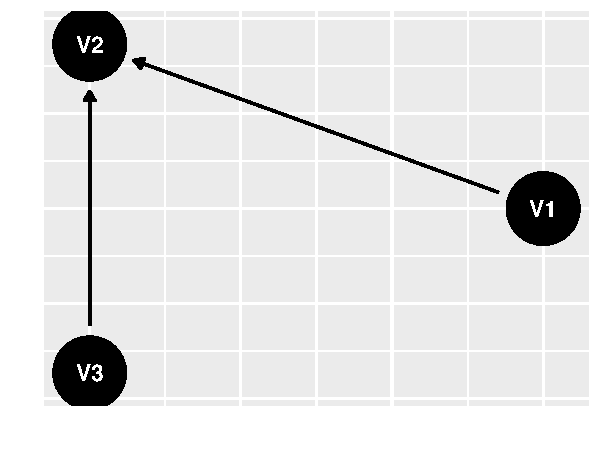
\includegraphics[width=\maxwidth]{figure/colisor-1} 

}

\caption[Ilustração de colisor]{Ilustração de colisor.}\label{fig:colisor}
\end{figure}

\end{knitrout}

Em um modelo de colisor 
a relação de dependência entre 
$V_1$ e $V_3$ é explicada pelos
resultados a seguir:

\begin{lemma}
 \label{lem:col-ind}
 Para qualquer probabilidade compatível com 
 o DAG na \cref{fig:colisor},
 $V_1 \ind V_3$.
\end{lemma}

\begin{proof}
 \begin{align*}
  f(v_1,v_3) 
  &= \int f(v_1, v_2, v_3) dv_2 \\
  &= \int f(v_1)f(v_3)f(v_2|v_1,v_3) dv_2 
  & \text{\cref{def:compativel}} \\
  &= f(v_1)f(v_3) \int f(v_2|v_1,v_3) dv_2 \\
  &= f(v_1)f(v_3)
 \end{align*}
\end{proof}

\begin{lemma}
 \label{lem:col-dep}
 Existe ao menos uma probabilidade compatível com
 o DAG na \cref{fig:colisor} tal que
 $V_1 \not\ind V_3 | V_2$.
\end{lemma}

\begin{proof}
 Considere que $V_1$ e $V_3$ são
 independentes e tem distribuição $\text{Bernoulli}(0.5)$.
 Além disso, $V_2 \equiv V_1+V_2$.
 Como $\P(V_3 = 1) = 0.5$ e
 $\P(V_3=1|V_1=1,V_2=2) = 1$, conclua que
 $V_1 \not\ind V_3 | V_2$.
\end{proof}

Combinando os \cref{lem:col-ind,lem:col-dep} vemos 
como utilizaremos confundidores num contexto causal.
Nestes casos, $V_1$ e $V_3$ serão causas comuns e independentes de $V_2$.
Uma vez que obtemos informação sobre o efeito comum, $V_2$,
$V_1$ e $V_3$ passam a ser associados.

Esse modelo pode ser contextualizado observando
a prevalência de doenças em uma determinada população 
\citep{Sackett1979}.
Considere que  $V_1$ e $V_3$ são 
indicadoras de que um indivíduo tem
doenças que ocorrem independentemente na população.
Além disso, $V_2$ é a indicadora de que 
o indíviduo foi hospitalizado, isto é,
$V_2$ é influeciado causalmente 
tanto por $V_1$ quanto por $V_3$.
Para facilitar as contas envolvidas,
desenvolveremos o exemplo com distribuições fictícias.
Considere que
$V_1$ e $V_3$ são independentes e
tem distribuição Bernoulli(0.05).
Além disso, quanto maior o número de doenças,
maior a probabilidade de o indíviduo ser hospitalizado.
Por exemplo,
$\P(V_2=1|V_1=0,V_3=0) = 0.01$,
$\P(V_2=1|V_1=0,V_3=1) = 0.1$,
$\P(V_2=1|V_1=1,V_3=0) = 0.1$, e
$\P(V_2=1|V_1=1,V_3=1) = 0.5$.

Com base nestas especificações, podemos
verificar se $V_1$ e $V_3$ estão associados
quando $V_2=1$. Para tal,
primeiramente calcularemos algumas
probabilidades conjuntas que serão úteis:
\begin{align}
 \label{eq:ex-col-1}
 \begin{cases}
  \P(V_1=0,V_2=1,V_3=0) &= 0.95 \cdot 0.01 \cdot 0.95 = 0.009025 \\
  \P(V_1=0,V_2=1,V_3=1) &= 0.95 \cdot 0.1 \cdot 0.05 = 0.0475 \\
  \P(V_1=1,V_2=1,V_3=0) &= 0.05 \cdot 0.1 \cdot 0.95 = 0.0475 \\
  \P(V_1=1,V_2=1,V_3=1) &= 0.05 \cdot 0.5 \cdot 0.05 = 0.00125
 \end{cases}
\end{align}

Com base nestes cálculos é possível obter
a prevalência da doença dentre os indivíduos hospitalizados:
\begin{align*}
 \P(V_1=1|V_2=1) 
 &= \frac{\P(V_1=1,V_2=1)}{\P(V_2=1)} \\
 &= \frac{0.0475 + 0.00125}{0.009025 + 0.0475 + 0.0475 + 0.00125} 
 & \text{\cref{eq:ex-col-1}} \\
 &\approx 0.46
\end{align*}

Finalmente,
\begin{align*}
 \P(V_1 = 1|V_2 = 1, V_3 = 1)
 &= \frac{\P(V_1=1,V_2=1,V_3=1)}{\P(V_2=1,V_3=1)} \\
 &= \frac{\P(V_1=1,V_2=1,V_3=1)}
 {\P(V_1=0,V_2=1,V_3=1) + \P(V_1=1,V_2=1,V_3=1)} \\
 &= \frac{0.00125}{0.0475 + 0.00125} & \text{\cref{eq:ex-col-1}} \\
 &\approx 0.26 
\end{align*}

Como $\P(V_1=1|V_2=1) = 0.46 \neq 0.26 \approx \P(V_1=1|V_2=1,V_3=1)$,
verificamos que $V_1$ não é independente de $V_3$ dado $V_2$.
De fato, ao observar que um indivíduo está hospitalizado e
tem uma das doenças, a probabilidade de que ele tenha
a outra doença é inferior àquela obtida se soubéssemos apenas
que o indivíduo está hospitalizado.

Esta observação 
não implica que uma doença tenha influência causal sobre a outra.
Note que a frequência de hospitalização aumenta 
drasticamente quando um indivíduo tem ao menos uma das doenças.
Além disso, cada uma das doenças é relativamente rara na população geral.
Assim, dentre os indíviduos hospitalizados,
a frequência daqueles que tem somente uma das doenças é
maior do que seria caso as doenças não estivessem associadas.
Quando fixamos o valor de uma consequência comum (hospitalização),
as causas (doenças) passam a ser associadas.
Esta associação não significa que,
infectar um indivíduo com uma das doenças
reduz a probabilidade que ele tenha a outra.

\subsection{Modelo Estrutural Causal (Structural Causal Model)}

Com base nos conceitos abordados anteriormente,
finalmente podemos definir formalmente
o Modelo Estrutural Causal (SCM):

\begin{definition}
 \label{def:scm}
 Um SCM é um par $(\sG,f)$ tal que
 $\sG = (\sV, \sE)$ é um DAG (\cref{def:dag}) e
 $f$ é uma função de densidade sobre $\sV$
 compatível com $\sG$ (\cref{def:compativel}).
 Neste caso, é comum chamarmos $\sG$ de
 \textbf{grafo causal} do SCM $(\sG,f)$.
\end{definition}

Note pela \cref{def:scm} que
um SCM é formalmente um modelo probabilístico em um DAG.
O principal atributo de um SCM que 
o diferencia de um modelo probabilístico genérico em um DAG é
como o interpretamos.
Existe uma aresta de $V_1$ em $V_2$ em um SCM
se e somente se $V_1$ é uma causa direta de $V_2$.

No próximo capítulo estudaremos consequências desta interpretação causal.
Contudo, antes disso, a próxima seção desenvolverá
um resultado fundamental de modelos probabilísticos em DAGs que
será fundamental nos capítulos posteriores.

\subsection{Exercícios}

\begin{exercise}
 Em um DAG, $\sG = (\sV, \sE)$,
 Considere que $Anc^*(\V) \subseteq \sV$ é
 definido como o menor conjunto tal que
 $\V \subseteq Anc^*(\V)$ e,
 se $V \in Anc^*(\V)$, então
 $Pa(V) \subseteq Anc^*(\V)$.
 Prove que $Anc(\V) \equiv Anc^*(\V)$.
\end{exercise}

\begin{exercise} 
 Prove o \cref{lem:anc}.
\end{exercise}

\begin{exercise}
 \label{lemma:anc_fact}
 Prove que se $\Z$ é ancestral, então
 $f(\Z) = \prod_{Z \in \Z}f(Z|Pa(Z))$. 
\end{exercise}

\begin{exercise}
 Sejam $\sG_1 = (\sV, \sE_1)$ e
 $\sG_2 = (\sV, \sE_2)$ grafos
 tais que $\sE_1 \subseteq \sE_2$.
 Prove que se 
 $f$ é compatível com $\sG_2$, então 
 $f$ é compatível com $\sG_1$.
\end{exercise}

\begin{exercise}
 Prove o \cref{lem:compativel-equiv}.
\end{exercise}

\begin{exercise}
 Prove o \cref{lem:anc_fat}.
\end{exercise}

\begin{exercise}
 Considere que $(X_1,X_2)$ são independentes e
 tais que $\P(X_i=1)=\P(X_i=-1)=0.5$.
 Além disso, $Y \equiv X_1 \cdot X_2$.
 \begin{enumerate}[label=(\alph*)]
  \item Desenhe um DAG compatível
  com as relações de independência dadas pelo enunciado.
  \item Prove que $Y$ e $X_1$ são independentes.
  Isso contradiz sua resposta para o item anterior?
 \end{enumerate}
\end{exercise}

\begin{exercise}
 Para cada um dos modelos de confundidor, cadeia e colisor,
 dê exemplos de situações práticas em que este modelo é razoável.
\end{exercise}

\begin{exercise}
 Considere que, dado $T$, $X_1,\ldots,X_n$ são i.i.d. e
 $X_i|T \sim \text{Bernoulli}(T)$. Além disso,
 $T \sim \text{Beta}(a,b)$.
 \begin{enumerate}[label=(\alph*)]
  \item Seja $f(t,x_1,\ldots,x_n)$ dada pelo enunciado.
  Exiba um DAG, $\sG$, tal que $f$ é compatível com $\sG$.
  \item $(X_1,\ldots,X_n)$ são independentes?
  \item Determine $f(x_1,\ldots,x_n)$.
 \end{enumerate}
\end{exercise}

\begin{exercise}
 Exiba um exemplo em que $V_1$, $V_2$, $V_3$ sejam binárias,
 que $V_2$ seja um colisor e que, além disso,
 $Corr[V_1,V_3|V_2=1] > 0$.
\end{exercise}

\begin{exercise}
 Seja $\sV = (V_1, V_2, V_3)$
 Exiba um exemplo de $f$ sobre $\sV$ e
 grafos $\sG_1$ e $\sG_2$ sobre $\sV$ tais que
 $\sG_1 \neq \sG_2$ e
 $f$ é compatível tanto com $\sG_1$ 
 quanto com $\sG_2$.
\end{exercise}

\begin{exercise}
 Seja $f$ uma densidade arbitrária sobre $\sV = (V_1,\ldots,V_n)$.
 Exiba um DAG sobre $\sV$, $\sG$,
 tal que $f$ é compatível com $\sG$.
\end{exercise}

\begin{exercise}
 Exiba um exemplo em que $V_2$ é um colisor 
 entre $V_1$ e $V_2$, 
 $V_4$ tem como único pai $V_2$ e
 $V_1$ e $V_3$ são dependentes dado $V_4$.
\end{exercise}
